

%%%% ijcai09.tex

\typeout{IJCAI-09 Instructions for Authors}

% These are the instructions for authors for IJCAI-09.
% They are the same as the ones for IJCAI-07 with superficical wording
%   changes only.

\documentclass{article}
% The file ijcai09.sty is the style file for IJCAI-09 (same as ijcai07.sty).
\usepackage{ijcai09}
\usepackage{url}
\usepackage{graphicx}
\usepackage{listings}
\usepackage{subfigure}

% Use the postscript times font!
\usepackage{times}

% the following package is optional:
%\usepackage{latexsym} 

% Following comment is from ijcai97-submit.tex:
% The preparation of these files was supported by Schlumberger Palo Alto
% Research, AT\&T Bell Laboratories, and Morgan Kaufmann Publishers.
% Shirley Jowell, of Morgan Kaufmann Publishers, and Peter F.
% Patel-Schneider, of AT\&T Bell Laboratories collaborated on their
% preparation.

% These instructions can be modified and used in other conferences as long
% as credit to the authors and supporting agencies is retained, this notice
% is not changed, and further modification or reuse is not restricted.
% Neither Shirley Jowell nor Peter F. Patel-Schneider can be listed as
% contacts for providing assistance without their prior permission.

% To use for other conferences, change references to files and the
% conference appropriate and use other authors, contacts, publishers, and
% organizations.
% Also change the deadline and address for returning papers and the length and
% page charge instructions.
% Put where the files are available in the appropriate places.

\title{HTTP Redirect Attack}
\author{Robert Christensen, Phil Lundrigan, Mark Thueson\\
Department of Computer Science\\
University of Utah \\
robert.christensen@gmail.com, philiplundrigan@gmail.com, m\_thueson@hotmail.com}

\begin{document}

\maketitle

\begin{abstract}
We analyze a security vulnerability of redirecting clients from non secure
websites to secure websites.  A compromised person in the middle can easily
sniff packets exchanged between a client and a server.  When a server sends
redirects a client from an unsecured a man in the middle can replace this
message with an illegitimate version of the site, potentially compromising
the security of the clients security credentials.  The complexity of this
attack is found to be very easy to deploy.  Several methods to patch
this vulnerability are discussed.

%Your abstract should concisely answer the following three questions: 1) what problem are you addressing? 2) what approach are you taking to solve the problem? 3) what are your results?
\end{abstract}

\section{Introduction}
Many people when attempting to connect to a secure website, such as a banking website, simply enter the well-known web address such as {\em www.chase.com}. Users often assume the a connection will be established with the desired host.  If applicable, especially for banking sites, the user will assume the connection established between the web browser and server will be secured.  However, the web assumes unsecure connections such as http and will establish a secure https connection only when a special request is made (see figure \ref{fg:redirect}).  When the well known web address {\em www.chase.com} is requested, the web server will request the IP address of the {\em chase.com} server over DNS.  When the correct IP server address is known to the client, the client will request the web page at {\em http://www.chase.com}.  In order to migrate the user to a secure, encrypted version of the website, a redirect message is returned from the server to point the client the secure website {\em https://www.chase.com}.  This inherent redirect is subject to a number of different attacks; however this work focuses on the possibility of intercepting the redirect packet and instead servicing the initial http request with a mock site \cite{offpath} (see figure \ref{fg:attack}).  We will show that an adversary can setup a public access point and perform such an attack.  If more time were given various solutions would also be explored that would mitigate the possibility of such attacks.


\section{Related Work}
Many works that can be found about phishing schemes that perform similar attacks.  Most of these use techniques such as ARP cache or DNS cache poisoning to allow all network traffic to be routed through them, the most notable of these is \texttt{sslstrip}\cite{sslstrip}.  These tools however are mostly focused on changing the redirect message to contain a homograph-similar site name (such as {\em www.cha5e.com} etc.).

Other works discuss the correctness of even allowing an http redirect to point
to an https citing security gaps such as the ones used by the aforementioned
tools.

\section{Adversary Model}
This attack is demonstrated as a type of Man In The Middle attack.  An adversary can easily become a person in the middle by providing a public access point and allow anyone to connect to the internet via his connection.  Being the first hop in their connection, all packets are available to sniff and alter when desired.  The adversary would use a network packet filter to forward all normal traffic but would keep a listing of sites that it has doctored and replace all redirects to https versions of these sites with the doctored site.  This would present the victim with a website that appears to be the normal https site they are used to but would actually only be a normal http site with the correct address that they initially typed (as opposed to a homograph-similar address).  Many sites could easily be copied with enough fidelity to trick an unsuspecting user into thinking they were connected to the intended site.  Since many people are unaware of the difference between http and https the adversary would be able to acquire sensitive information from the victim such as usernames and passwords.

%%%%%%%%%% Figure %%%%%%%%%%
\begin{figure}[t]
\begin{center}

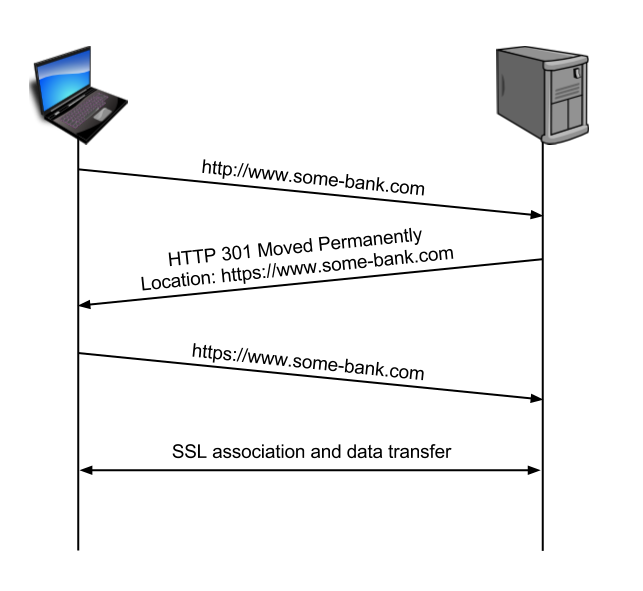
\includegraphics[width=2.3in]{normal_redirect.png} 
\caption{A typical HTTP redirect to switch from HTTP to HTTPS} 
\label{fg:redirect}

\end{center}
\end{figure}
%%%%%%%%%%%%%%%%%%%%%%%%

\section{Methodology}
We were unable to implement any solution to this problem but thought of a 
few ways one would go about implementing one.
One idea is to build a table into browsers that contains lists of sites that should always resolve using the https version instead of http.  This list could be maintained through browser updates and other methods.  However, the Internet can change very rapidly.  A website trying to migrate from an http site to an https site would not appear in the table until the browser is updated.  Many browsers are not updated frequently\cite{ie6countdown}, so much of the internet would remain vulnerable.

Any site that uses one time passwords can easily be protected against these types of attacks.  If a client is attempting to connect via an untrusted access point they can be issued a one time password via a secondary trusted authority that is registered to their account such as a cell phone.  This prevents the client from ever entering in their long term password and an adversary from acquiring any sensitive information.  While this does provide additional security it also makes authenticating harder on the user.  It also makes the assumption that a secure secondary authority is available.

Multiple stage authentication is an option that servers can provide to guard against these attacks as well.  To implement this the server would prompt the client for minimal information such as an account number or username.  The server can then issue challenges set by the client (such as personal questions) which allows the client to authenticate the server.  Only once these stages are complete would the server prompt for sensitive information such as a password.

Some people purpose the idea that the redirect message should be exchanged for an error message that prompts the user to manually contact the server via the https address.  This may thwart many problems similar to the one in this paper but also creates a less user friendly method because the process becomes less automated then it is today.

Ideally there would be a way to make it the networks responsibility so it could be done without bothering either the client or the server.  In order for this to occur major changes to the current network would have to be made.  Implementing IPSec or transitioning to Content Centric Networking would actually solve all attacks of this nature.

%%%%%%%%%% Figure %%%%%%%%%%
\begin{figure}[t]
\begin{center}

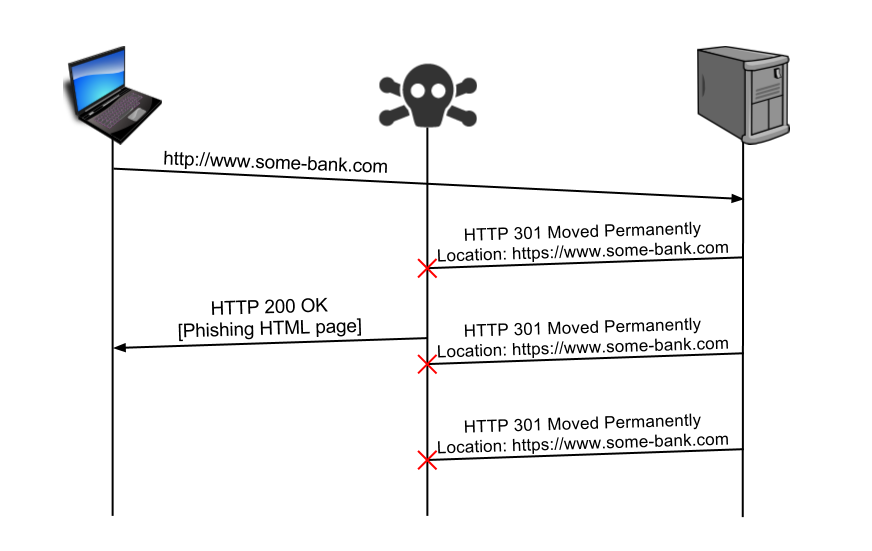
\includegraphics[width=3.1in]{redirect_attack.png} 
\caption{A HTTP Redirect attack} 
\label{fg:attack}

\end{center}
\end{figure}
%%%%%%%%%%%%%%%%%%%%%%%%

\section{Implementation / Experimentation}
For our experiments, we wanted to see how feasible it is to implement a HTTP redirect attack in a real computer system. To do this we used two libraries: \texttt{netfilter} \cite{netfilter} and \texttt{netfilter\_queue}\ cite{netfilterQueue}. These two libraries, along with modifying the IP tables of the Linux kernel, allowed us to receive packets and bring them from the kernel into user space. We also used part of the \texttt{wifu}\cite{wifu} framework to handle system callbacks when a packet arrives. By bringing the packet into user space, we were then able to write a program that filters a packet based on its IP address. 

To implement this attack, a "watch list" is kept to decide which IP addresses should be monitored. When a packet is received with an IP address that is on the "watch list" and it is a \texttt{HTTP 301 Moved Permanently} response, we change the packet payload to a pre-made phishing website. This can be done by locating the beginning of the TCP packet payload and overriding its contents with our own data. There are a few considerations that must be made for this attack to work. First, we know that the current payload will be relatively small since the packet is a HTTP redirect response. The packet's payload size must be adjusted to account for the larger size of the payload. Second, the TCP and IP checksum must be recalculated so that the transport layer will be able to validate the packet.

From this experience of building this attack we learned that although this attack is relatively straightforward, it was much harder to implement on a real system (though this could be due to our lack of experience). It took a lot of time and effort just to set up an environment where we could use \texttt{netfilter} and \texttt{netfilter\_queue} so that we could look at the packets. Once we had accomplished this, we still had many other problems to face. One thing we did not originally account for was that large websites have multiple IP addresses so a packet might not come from the same location between sessions. To solve this problem we used a "watch list", as mentioned above, to list out all the IP address it should monitor. Another problem we faced was when to block responses from the server. Originally we tried to block all communication between the client and server but quickly realized that the TCP connection needed to be made for this attack to work. To fix this problem we add the functionality to detect if the packet is a HTTP response by looking at the packet's payload. Only if the packet is a HTTP 301 response do we modify the packet.

The source code for this application can be viewed at {\em https://github.com/markthueson/network-security}.

\section{Conclusion}
The attack that we have explored as well as other similar attacks are quite wide in scope and variety; however each of them relies on the lack of security in the transport layer.  Until that base issue is resolved by implementing a security method many phishing attacks will remain a possibility.  Architectural solutions such as content centric networking ask too much of the backbone providers without enough incentive to perform the implementation.  Solutions such as one time passwords put more of a burden on the user making the experience more difficult or time consuming.  Other solutions such as implementing a browser database to track https sites simply have too much overhead.  Surely the best way to prevent such attacks is to educate the average user so they know what to look for when attempting to create secure connections; however this may be even less feasible many of the solutions proposed herein.

% Here is a reference to different bib formats:
%	http://en.wikibooks.org/wiki/LaTeX/Bibliography_Management
\bibliographystyle{plain}
\bibliography{ref}

\end{document}



